\documentclass[11pt, letterpaper]{article}
\usepackage{amsmath, amssymb}
\usepackage{hyperref}
\usepackage{booktabs}
\usepackage{enumitem}
\usepackage{xcolor}
\usepackage{geometry}
\usepackage{fancyhdr}
\usepackage{titlesec}
\usepackage{tcolorbox}
\usepackage{graphicx}
\usepackage{parskip}
\usepackage{caption}
\usepackage{tabularx}
\usepackage{pgfplots}
\pgfplotsset{compat=1.17}
\geometry{margin=1in}

\definecolor{courseblue}{HTML}{002452}
\definecolor{coursegold}{HTML}{FABD0F}
\definecolor{coursered}{HTML}{B90E31}
\definecolor{lightblue}{HTML}{E8EEF7}
\definecolor{lightgold}{HTML}{FEF8E3}

\hypersetup{colorlinks=true,linkcolor=courseblue,urlcolor=coursered}
\tcbuselibrary{skins}
\newtcolorbox{guidancebox}{enhanced,colback=lightblue,colframe=courseblue,
  sharp corners,leftrule=4pt,left=6pt,right=6pt,top=4pt,bottom=4pt}
\newtcolorbox{notebox}{enhanced,colback=lightgold,colframe=coursegold,
  sharp corners,leftrule=4pt,left=6pt,right=6pt,top=4pt,bottom=4pt}

\pagestyle{fancy}\fancyhf{}
\fancyhead[L]{\small\textcolor{courseblue}{\textbf{CISC 473 --- Deep Learning | Fall 2026}}}
\fancyhead[R]{\small\textcolor{courseblue}{Midterm Report}}
\fancyfoot[C]{\small\thepage}
\renewcommand{\headrulewidth}{0.4pt}
\titleformat{\section}{\large\bfseries\color{courseblue}}{}{0em}{}[\titlerule]
\titleformat{\subsection}{\normalsize\bfseries\color{courseblue}}{}{0em}{}

\begin{document}

{\centering
  {\Large\textbf{CISC 473: Deep Learning --- Midterm Report}}\par\vspace{0.5em}
  {\large\textit{P22: Cross-Architecture Knowledge Distillation}}\par\vspace{0.4em}
  \textbf{Group Members:}\par
  Lee Xuan \quad 20630324 \quad (Role: Project Lead)\par
  Fong Yee Xin \quad 20629927 \quad (Role: Engineering Lead)\par
  \textbf{GitHub Repository:} \url{https://github.com/l33zard/cakd.git}\par\vspace{0.3em}
  \textbf{Date:} October 22, 2026\par\vspace{0.4em}
  \rule{\linewidth}{0.4pt}
}

\section{Abstract}

Knowledge distillation (KD) compresses a large teacher network into a compact
student, but most feature-level KD methods assume teacher and student share an
architectural family. We study the harder cross-architecture case of a
convolutional ResNet-50 teacher and a DeiT-Tiny vision-transformer student on
CIFAR-100, where spatial feature maps must be related to patch-token
sequences. To date we have implemented a deterministic CIFAR-100 pipeline
(45k/5k/10k train/validation/test split), CIFAR-adapted ResNet-50 and
DeiT-Tiny models, a shared training and evaluation engine, and resumable
training scripts for the teacher and for the from-scratch student baseline.
After 100 epochs the ResNet-50 teacher reaches 75.35\% top-1 and 93.47\%
top-5 test accuracy (single seed), below the reference result discussed in the
proposal under a longer training schedule.
The from-scratch DeiT-Tiny student has completed an initial four-epoch
preliminary run (25.24\% validation top-1), confirming that the supervised
student pipeline runs end to end; its completed run will establish the lower
bound that distillation must improve on. The next stages are vanilla KD,
layer-wise CKA measurement, and the proposed projected-feature alignment loss.

\section{Introduction and Problem Statement}

Edge deployment favours small models, and vision transformers are increasingly
the architecture of choice for compact students, yet the strongest teachers
available for small-image tasks are often CNNs. Logit-only KD [1,3] transfers
across architectures but discards the teacher's intermediate knowledge, while
feature-level methods [2,4,5,7] were designed for CNN-to-CNN pairs whose
feature maps are directly comparable. A CNN produces a $C\times H\times W$
spatial map and a ViT produces an $N\times D$ token sequence, so feature
transfer between them needs an explicit alignment step.

\textbf{Research question.} \emph{Does aligning projected intermediate CNN
features with ViT patch tokens, using a CKA-based loss, give a DeiT-Tiny
student accuracy gains on CIFAR-100 beyond logit-only KD, at unchanged
inference cost, and is any gain accompanied by higher teacher--student CKA
similarity?}

\textbf{Scope changes since the proposal.} Following instructor feedback, we
narrowed the project to one cross-architecture pair: ResNet-50 teacher
$\rightarrow$ DeiT-Tiny student on CIFAR-100. The required progression is the
data pipeline, teacher, supervised student, vanilla KD, CKA measurement,
projected CKA alignment, and focused ablations. CRD, ReviewKD, DKD,
TinyImageNet, the ResNet-110 $\rightarrow$ MobileNetV2 pair, and attention-map
alignment are out of scope for this project.

\section{Related Work (Updated)}

\textbf{Logit-based distillation.} Hinton et al.~[1] train the student to match
the teacher's temperature-softened outputs, exposing the ``dark knowledge'' in
non-target class probabilities. DKD~[3] shows that the classical loss couples
non-target knowledge to the teacher's target confidence and decouples the two
terms, matching feature-based methods at logit-only cost. Because they act only
on output distributions, both transfer unchanged across architectures, which
makes vanilla KD our base objective and DKD the strongest logit-only reference.

\textbf{Feature-based distillation.} FitNets~[5] introduced intermediate
``hints'' with a learnable regressor to reconcile channel widths; our projection
module generalises this regressor from a channel mismatch to a map-versus-token
mismatch. CRD~[2] maximises a contrastive bound on teacher--student mutual
information over pooled embeddings, ReviewKD~[4] lets deeper student stages
attend to shallower teacher stages, and RKD~[7] transfers pairwise distance and
angle structure, which is insensitive to representation dimensionality. All
were developed and evaluated almost entirely on CNN pairs.

\textbf{Cross-architecture distillation.} DeiT~[9] trains a ViT student from a
CNN teacher (RegNetY) through a dedicated distillation token and finds that a
convolutional teacher outperforms a transformer teacher, suggesting the CNN's
inductive bias is itself useful knowledge; however, it distils logits only and
modifies the student architecture with an extra token. Liu et al.~[11] project
CNN features into a transformer-like space with partially cross-attentive and
group-wise linear projectors, and OFA-KD~[12] projects intermediate features of
heterogeneous students into the logit space and distils there, reporting gains
on CIFAR-100 and ImageNet across CNN, ViT and MLP pairs. Our approach differs in
aligning token-level representations directly with a CKA objective [6], adding
no tokens to the student, and using CKA as a diagnostic of where transfer
succeeds. These papers provide context for heterogeneous distillation, but
they are not implemented as baselines in the narrowed project.

\begin{center}
\begin{tabular}{llp{4.2cm}p{4.2cm}}
\toprule
\textbf{Method} & \textbf{Year} & \textbf{Key idea} & \textbf{Relation to our work} \\
\midrule
Vanilla KD [1] & 2015 & Match temperature-softened logits & Base loss term; first baseline \\
FitNets [5] & 2015 & $L_2$ hint loss with learnable regressor & Ancestor of our projection module \\
CKA [6] & 2019 & Invariant similarity of representations & Diagnostic and alignment loss \\
CRD [2] & 2020 & Contrastive teacher--student MI bound & Feature-level baseline (CNN pairs) \\
ReviewKD [4] & 2021 & Cross-stage review of teacher features & Motivates layer-pair ablation \\
DeiT [9] & 2021 & Distillation token, CNN teacher $\rightarrow$ ViT & Logit-only CNN$\rightarrow$ViT reference \\
DKD [3] & 2022 & Decoupled target / non-target KD & Strongest logit-only baseline \\
OFA-KD [12] & 2023 & Distil heterogeneous features in logit space & Closest cross-architecture competitor \\
\bottomrule
\end{tabular}
\end{center}

\section{Methodology}

\subsection{Model Architecture}

\textbf{Teacher.} ResNet-50 [8] from \texttt{torchvision}, randomly initialized
(no pre-trained weights). For $32\times32$ inputs the $7\times7$ stride-2 stem
is replaced by a $3\times3$ stride-1 convolution, the initial max-pool is
removed, and the classifier outputs 100 classes. The \texttt{layer3} output is
a $1024\times8\times8$ map. The implementation contains 23,705,252 trainable
parameters.

\textbf{Student.} DeiT-Tiny [9] from \texttt{timm}, randomly initialised, with
the standard 192-dimensional embedding, 12 blocks and 3 heads, but with input
size 32 and patch size 4. This gives an $8\times8$ grid of 64 patch tokens plus
a class token (sequence $65\times192$). The implementation contains
5,380,132 trainable parameters.

\textbf{Planned alignment module (not yet implemented).} The primary pair is
ResNet layer3 $\rightarrow$ DeiT transformer block 8. The teacher's
$8\times8$ \texttt{layer3} map is reshaped from
$B\times1024\times8\times8$ to $B\times64\times1024$ and passed through a
learnable linear projection $1024\to192$. The student representation uses
the 64 patch tokens after block 8; the CLS token is excluded. Both projected
representations are reshaped to $(B\cdot64)\times192$, treating patch/token
positions across the minibatch as observations and embedding coordinates as
features. We use centered linear CKA,
\[
\operatorname{CKA}(X,Y)=
\frac{\lVert X^{\mathsf T}Y\rVert_F^2}
{\lVert X^{\mathsf T}X\rVert_F\,\lVert Y^{\mathsf T}Y\rVert_F+\varepsilon},
\qquad \mathcal{L}_{\mathrm{align}}=1-\operatorname{CKA}(X,Y).
\]
The total proposed student objective is
\[
\mathcal{L} = (1-\alpha)\,\mathcal{L}_{\text{CE}}
            + \alpha\,\tau^{2}\,\mathrm{KL}\!\left(\sigma(z_T/\tau)\,\Vert\,\sigma(z_S/\tau)\right)
            + \beta\,\bigl(1-\mathrm{CKA}(P(F_T),\,F_S)\bigr),
\]
where $P$ is the projection and $F_S$ contains patch tokens only. The
projection is discarded after training, so inference cost is unchanged. The
focused layer-pair ablation compares early layer2 $\rightarrow$ block4,
middle layer3 $\rightarrow$ block8, and late layer4 $\rightarrow$ block12.
These pairs are not all shape-compatible before adaptation. For the early pair,
the teacher output has shape $B\times512\times16\times16$; it is bilinearly
resized to $8\times8$, flattened to $B\times64\times512$, and projected with
a separate $512\to192$ linear layer. The middle pair naturally produces
$B\times64\times1024$ before its $1024\to192$ projection. For the late pair,
the $B\times2048\times4\times4$ teacher output is bilinearly resized to
$8\times8$, flattened to $B\times64\times2048$, and projected with a separate
$2048\to192$ linear layer. After these operations, every teacher pair produces
$B\times64\times192$, matching the student's 64 patch tokens; both are then
reshaped to $(B\cdot64)\times192$ for CKA.

\subsection{Training Setup}

{\small
\begin{tabularx}{\linewidth}{@{}p{0.22\linewidth}XX@{}}
\toprule
\textbf{Hyperparameter} & \textbf{Teacher (ResNet-50)} & \textbf{Student (DeiT-Tiny, scratch)} \\
\midrule
Optimiser & SGD, momentum 0.9 & AdamW \\
Learning rate & 0.1, cosine annealing & $3\times10^{-4}$, cosine decay (no warm-up in the final protocol) \\
Weight decay & $5\times10^{-4}$ & 0.05 \\
Batch size & 128 & 128 \\
Epochs & 100 & 100 \\
Loss function & Cross-entropy & Cross-entropy \\
Data augmentation & Random crop (pad 4), horizontal flip & Same \\
Random seeds used & 42 initially; 123 and 999 planned & 42 initially; 123 and 999 planned \\
\bottomrule
\end{tabularx}
}

The checkpoint with the best validation top-1 accuracy is kept and evaluated
once on the test set. The trained teacher checkpoint
(\texttt{teacher\_best.pt}) and metric logs are available at
\url{https://drive.google.com/drive/folders/1J2HeM9IKQTrtBiroXC0C_Mx8FZVZoYu9?usp=sharing};
see the repository README for usage. Training scripts save the best validation
checkpoint and epoch-level CSV metrics. Both scripts support resuming from a
checkpoint, restoring the model, optimiser, and learning-rate schedule state;
smoke-test outputs are used only for pipeline verification and are not
presented as research results.

\subsection{Dataset and Preprocessing}

CIFAR-100 [10]: 60{,}000 $32\times32$ colour images in 100 balanced classes.
The official 50{,}000-image training set is split deterministically (split seed
42) into 45{,}000 training and 5{,}000 validation images; the official
10{,}000-image test set is used only for final evaluation. Images are
normalised with per-channel CIFAR-100 mean and standard deviation; training
images additionally receive a random $32\times32$ crop after 4-pixel padding
and a random horizontal flip, while validation and test images are not
augmented. Classes are balanced, so no re-weighting is applied.

\textbf{Evaluation protocol.} Top-1 and top-5 accuracy on the test set, reported
as mean $\pm$ std over 3 seeds, together with parameter count and training time.

\section{Preliminary Results}

\subsection{Baseline Reproduction}

\begin{notebox}
\textbf{Target:} Match the published number within 1--2\% before proceeding
to your proposed modification.
\end{notebox}

\begin{center}
\begin{tabular}{lccc}
\toprule
\textbf{Model} & \textbf{Top-1 (\%)} & \textbf{Top-5 (\%)} & \textbf{Params} \\
\midrule
ResNet-50 teacher, ours (100 ep., test) & 75.35 & 93.47 & 23,705,252 \\
DeiT-Tiny student, scratch (4/100 ep., val.) & 25.24$^\dagger$ & 57.12$^\dagger$ & 5,380,132 \\
\bottomrule
\end{tabular}
\captionof{table}{Preliminary results on CIFAR-100. Our results are from a
single seed (42); the remaining two seeds are scheduled for Weeks 7--8, after
which we will report mean $\pm$ std. $^\dagger$Validation accuracy after 4 of
100 epochs, not a final result. These are preliminary single-seed results and
must be rerun or accompanied by their saved logs before the final report.}
\end{center}

\subsection{Qualitative Analysis}

\begin{figure}[h]
  \centering
  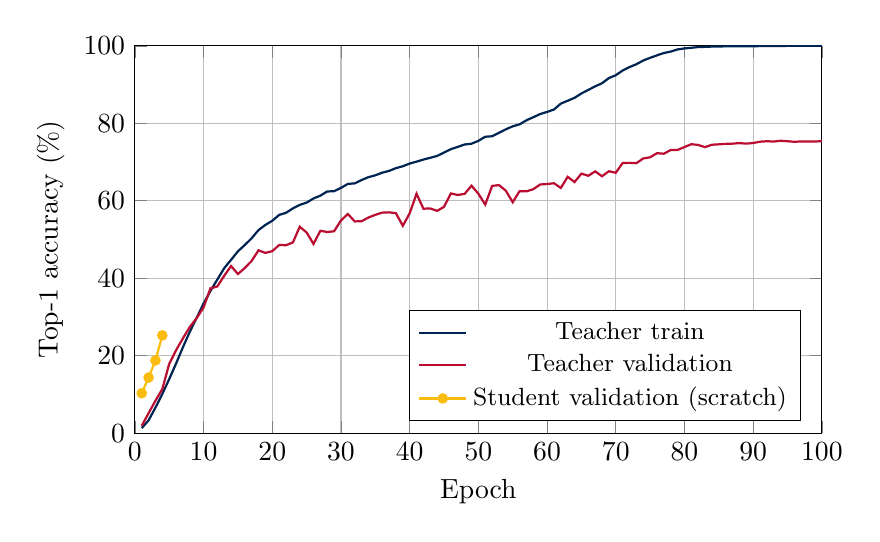
\begin{tikzpicture}
  \begin{axis}[width=0.85\linewidth,height=6.5cm,xlabel={Epoch},ylabel={Top-1 accuracy (\%)},
    xmin=0,xmax=100,ymin=0,ymax=100,grid=major,legend pos=south east,legend style={font=\small}]
\addplot[thick,color=courseblue] coordinates {(1,1.29) (2,3.30) (3,6.59) (4,10.12) (5,13.94) (6,17.97) (7,22.18) (8,26.18) (9,29.79) (10,33.46) (11,36.71) (12,39.64) (13,42.57) (14,44.73) (15,46.93) (16,48.57) (17,50.32) (18,52.42) (19,53.76) (20,54.82) (21,56.34) (22,56.88) (23,58.01) (24,58.93) (25,59.51) (26,60.58) (27,61.31) (28,62.39) (29,62.46) (30,63.32) (31,64.34) (32,64.48) (33,65.34) (34,66.09) (35,66.56) (36,67.24) (37,67.70) (38,68.41) (39,68.90) (40,69.60) (41,70.09) (42,70.63) (43,71.09) (44,71.57) (45,72.44) (46,73.31) (47,73.90) (48,74.52) (49,74.72) (50,75.46) (51,76.52) (52,76.65) (53,77.53) (54,78.44) (55,79.21) (56,79.72) (57,80.77) (58,81.57) (59,82.38) (60,82.93) (61,83.54) (62,85.08) (63,85.81) (64,86.57) (65,87.70) (66,88.62) (67,89.53) (68,90.34) (69,91.67) (70,92.40) (71,93.62) (72,94.51) (73,95.25) (74,96.21) (75,96.90) (76,97.54) (77,98.14) (78,98.51) (79,99.07) (80,99.32) (81,99.49) (82,99.68) (83,99.73) (84,99.80) (85,99.82) (86,99.87) (87,99.88) (88,99.88) (89,99.90) (90,99.90) (91,99.92) (92,99.92) (93,99.94) (94,99.94) (95,99.99) (96,99.98) (97,99.99) (98,100.00) (99,99.99) (100,100.00)};
\addlegendentry{Teacher train}
\addplot[thick,color=coursered] coordinates {(1,1.88) (2,5.14) (3,8.38) (4,11.38) (5,17.88) (6,21.40) (7,24.48) (8,27.42) (9,29.70) (10,32.42) (11,37.36) (12,37.86) (13,40.60) (14,43.14) (15,41.08) (16,42.62) (17,44.46) (18,47.20) (19,46.52) (20,46.98) (21,48.56) (22,48.52) (23,49.22) (24,53.28) (25,51.80) (26,48.84) (27,52.24) (28,51.92) (29,52.12) (30,54.90) (31,56.58) (32,54.66) (33,54.70) (34,55.66) (35,56.36) (36,56.92) (37,57.00) (38,56.78) (39,53.52) (40,56.74) (41,61.80) (42,57.94) (43,58.00) (44,57.38) (45,58.42) (46,61.88) (47,61.48) (48,61.78) (49,63.88) (50,61.82) (51,59.00) (52,63.82) (53,64.04) (54,62.58) (55,59.60) (56,62.48) (57,62.42) (58,62.98) (59,64.20) (60,64.30) (61,64.52) (62,63.30) (63,66.18) (64,64.82) (65,67.00) (66,66.44) (67,67.58) (68,66.32) (69,67.62) (70,67.22) (71,69.74) (72,69.78) (73,69.70) (74,70.92) (75,71.22) (76,72.28) (77,72.14) (78,73.10) (79,73.12) (80,73.86) (81,74.60) (82,74.40) (83,73.84) (84,74.46) (85,74.56) (86,74.68) (87,74.74) (88,74.88) (89,74.74) (90,74.90) (91,75.24) (92,75.36) (93,75.28) (94,75.48) (95,75.36) (96,75.22) (97,75.30) (98,75.28) (99,75.28) (100,75.40)};
\addlegendentry{Teacher validation}
\addplot[thick,color=coursegold,mark=*,mark size=1.5pt] coordinates {(1,10.30) (2,14.34) (3,18.76) (4,25.24)};
\addlegendentry{Student validation (scratch)}
  \end{axis}
  \end{tikzpicture}
  \caption{Top-1 accuracy per epoch on CIFAR-100. The ResNet-50 teacher's
  training accuracy reaches $\approx$100\% while validation accuracy plateaus at
  $\approx$75\% (best 75.48\% at epoch 94), showing a large generalisation gap.
  The DeiT-Tiny curve shows only the initial four-epoch preliminary run.}
  \label{fig:qual}
\end{figure}

\subsection{Discussion}

\textbf{Teacher reproduction.} Our teacher reaches 75.35\% test top-1, about 4
points below the reference value cited in the proposal, so it does not yet
meet the original reproduction target. The most likely causes are the shorter
100-epoch budget and differences between published and local training recipes.
A teacher that is substantially stronger than the student remains useful for
the planned distillation comparison, but the teacher gap must be reported when
interpreting KD gains.

\textbf{Overfitting.} Training accuracy reaches 99.99\% and training loss falls
to 0.007, while validation accuracy plateaus near 75\% from about epoch 85
onwards (Fig.~\ref{fig:qual}). The teacher has effectively memorised the
45k-image training set with only crop and flip augmentation. Stronger
regularisation (e.g.\ mixup or longer schedules) could narrow this gap, though
we prioritise the distillation experiments over further tuning the teacher.

\textbf{Student.} After four epochs the student reaches 25.24\% validation
top-1. This is an incomplete preliminary run, so no conclusion about final
student accuracy or distillation gains can be drawn yet.
Vision transformers trained from scratch on small datasets are known to
underperform CNNs because they lack a locality prior [9]; the size of the
final teacher--student gap is the headroom that distillation must recover.

\section{Challenges and Adaptations}

\textbf{Compute interruptions.} Training uses the Google Colab free tier, whose
sessions end after roughly 12 hours or on inactivity, deleting anything stored
on the runtime's local disk. We moved checkpoints and metric logs to Google
Drive and added a \texttt{--resume} option that restores model, optimiser and
learning-rate schedule from the last best checkpoint, which let the 100-epoch
teacher run complete across several sessions.

\textbf{Correct resumption.} An early version restarted the cosine schedule from
the wrong epoch after a resume and mixed zero- and one-based epoch numbers; we
fixed both so a resumed run follows the same learning-rate curve as an
uninterrupted one. Because only the best checkpoint is saved, resuming can
repeat a few epochs and append duplicate rows to the metrics log; these are
removed before plotting.

\textbf{Feature-shape compatibility.} Choosing patch size 4 for DeiT-Tiny gives
an $8\times8$ token grid with 64 patch tokens. The primary layer3 $\rightarrow$
block8 pair already has this spatial resolution, so it needs no interpolation.
The early layer2 output is $16\times16$ with 256 spatial positions, while the
late layer4 output is $4\times4$ with 16 positions; neither can be compared
directly with the student's 64 tokens. Both ablation maps are therefore
bilinearly resized to $8\times8$ and use their own channel projection before
flattening to $(B\cdot64)\times192$. We verify the raw model shapes with
temporary forward hooks in \texttt{src/models.py}.

\textbf{Timeline.} We are behind the proposal schedule, which placed vanilla
KD in Week 3, CRD in Week 4, DKD in Week 5 and ReviewKD and CKA in Week 6. So
far the data pipeline, both models, the shared training engine, the complete
100-epoch teacher run and the first 4 epochs of the scratch student are done.
The 100-epoch teacher alone consumed several free-tier GPU sessions, and the
student run paused when the Colab quota was exhausted. We are moving
remaining training to Kaggle (30 GPU-hours per week) in addition to Colab and
re-ordering the plan below so the core CNN$\rightarrow$ViT comparison is
completed first.

\subsection{Updated Week 7--10 Plan}

\small
\begin{tabularx}{\linewidth}{@{}p{0.7cm}Xp{1.2cm}@{}}
\toprule
\textbf{Week} & \textbf{Tasks} & \textbf{Responsible} \\
\midrule
7 & Finish scratch student (100 epochs); implement vanilla KD; run temperature and loss-weight screening; implement layer-wise CKA tooling & All \\
8 & Implement projected-CKA alignment; run the specified layer-pair and loss-weight ablations & All \\
9 & Run selected configurations with seeds 42, 123, and 999; produce CKA comparisons and efficiency analysis & All \\
10 & Final report, presentation, single-command reproduction and README \textbf{(Final due)} & All \\
\bottomrule
\end{tabularx}

\section{Preliminary Novel Contribution (Optional Bonus)}

The planned contribution is a reproducible CKA-based study of CNN-to-ViT
distillation. We will compare the primary layer pair and the early/middle/late
ablation pairs, then test whether higher CKA similarity is associated with
higher classification accuracy. This contribution remains prospective until
the alignment implementation and experiments are complete.

\section{AI Tool Disclosure}

AI assistance was used to inspect the repository, suggest report structure and
wording, and help identify implementation and documentation issues. The group
remains responsible for the code, experiments, results, interpretation, and
final verification of this report.

\section{Contribution Declaration}

\small
\begin{tabularx}{\linewidth}{@{}p{2.3cm}Xp{0.8cm}@{}}
\toprule
\textbf{Member} & \textbf{Contributions (this period)} & \textbf{\%} \\
\midrule
Lee Xuan & Project coordination; literature review; scope refinement; teacher training and evaluation; preliminary-results analysis; report and presentation preparation & 50\% \\
Fong Yee Xin & CIFAR-100 data pipeline; ResNet-50 and DeiT-Tiny implementation; shared training/evaluation engine; student and teacher scripts; checkpointing and reproducibility support & 50\% \\
\bottomrule
\end{tabularx}

\section{References}

\begin{enumerate}[label={[\arabic*]},leftmargin=*]
  \item Hinton, G., Vinyals, O., and Dean, J., 2015. ``Distilling the Knowledge in a Neural Network.'' \textit{NeurIPS Deep Learning and Representation Learning Workshop}. arXiv:1503.02531.
  \item Tian, Y., Krishnan, D., and Isola, P., 2020. ``Contrastive Representation Distillation.'' \textit{ICLR}. arXiv:1910.10699.
  \item Zhao, B., Cui, Q., Song, R., Qiu, Y., and Liang, J., 2022. ``Decoupled Knowledge Distillation.'' \textit{CVPR}. arXiv:2203.08679.
  \item Chen, P., Liu, S., Zhao, H., and Jia, J., 2021. ``Distilling Knowledge via Knowledge Review.'' \textit{CVPR}. arXiv:2104.09044.
  \item Romero, A., Ballas, N., Kahou, S. E., Chassang, A., Gatta, C., and Bengio, Y., 2015. ``FitNets: Hints for Thin Deep Nets.'' \textit{ICLR}. arXiv:1412.6550.
  \item Kornblith, S., Norouzi, M., Lee, H., and Hinton, G., 2019. ``Similarity of Neural Network Representations Revisited.'' \textit{ICML}. arXiv:1905.00414.
  \item Park, W., Kim, D., Lu, Y., and Cho, M., 2019. ``Relational Knowledge Distillation.'' \textit{CVPR}. arXiv:1904.05068.
  \item He, K., Zhang, X., Ren, S., and Sun, J., 2016. ``Deep Residual Learning for Image Recognition.'' \textit{CVPR}. arXiv:1512.03385.
  \item Touvron, H., Cord, M., Douze, M., Massa, F., Sablayrolles, A., and J\'egou, H., 2021. ``Training Data-Efficient Image Transformers \& Distillation through Attention.'' \textit{ICML}. arXiv:2012.12877.
  \item Krizhevsky, A., 2009. ``Learning Multiple Layers of Features from Tiny Images.'' Technical report, University of Toronto.
  \item Liu, Y., Cao, J., Li, B., Hu, W., Ding, J., and Li, L., 2022. ``Cross-Architecture Knowledge Distillation.'' \textit{ACCV}. arXiv:2207.05273.
  \item Hao, Z., Guo, J., Han, K., Tang, Y., Hu, H., Wang, Y., and Xu, C., 2023. ``One-for-All: Bridge the Gap Between Heterogeneous Architectures in Knowledge Distillation.'' \textit{NeurIPS}. arXiv:2310.19444.
\end{enumerate}

\end{document}
